\documentclass{article}
\usepackage{geometry}
\geometry{a4paper, landscape, margin=1.5cm}
\usepackage{graphicx}
\graphicspath{ {images/} }
\usepackage{listings}
\usepackage{xcolor}

\definecolor{codegreen}{rgb}{0,0.6,0}
\definecolor{codegray}{rgb}{0.5,0.5,0.5}
\definecolor{codepurple}{rgb}{0.58,0,0.82}
\definecolor{backcolour}{rgb}{1,1,1}

\lstdefinestyle{mystyle}{
    backgroundcolor=\color{backcolour},   
    commentstyle=\color{codegreen},
    keywordstyle=\color{magenta},
    numberstyle=\tiny\color{codegray},
    stringstyle=\color{codepurple},
    basicstyle=\ttfamily\footnotesize,
    breakatwhitespace=false,         
    breaklines=true,                 
    captionpos=b,                    
    keepspaces=true,                 
    numbers=left,                    
    numbersep=5pt,                  
    showspaces=false,                
    showstringspaces=false,
    showtabs=false,                  
    tabsize=2
}

\lstset{style=mystyle}

\author{\Large submitted by\\ Arghya Bandyopadhyay\\
    	RollNo. 20CS4103\\}
\title{\begin{center}
       \bfseries\Large
    	Assignment 3\\
    	Of\\
    	Network \& Distributed System Lab (CS2051)\\
        Masters of Technology in Computer Science And Engineering\\
    	\vskip1cm
    	submitted to\\
    	Dr Sujoy Saha\\
    	Assistant Professor\\
    	\&\\
    	Dr Suvrojit Das\\
    	Associate Professor\\
    	Dept. of CSE\\
    	\vskip1cm
    	
\includegraphics[width=4cm]{NITDGP}\\
    	National Institute of Technology, Durgapur\\
    \end{center}}
\date{14 June 2021}
\begin{document}
\maketitle
\pagebreak

\textbf{Objective:} Implement naïve flow control mechanism using stop \& wait protocol. Transfer
files (Text, Image, Audio, Video) using TCP and UDP protocol. If during the connection
suddenly connection is terminated then you have start ones again, it simply resume the
process not start from being.

\begin{center}
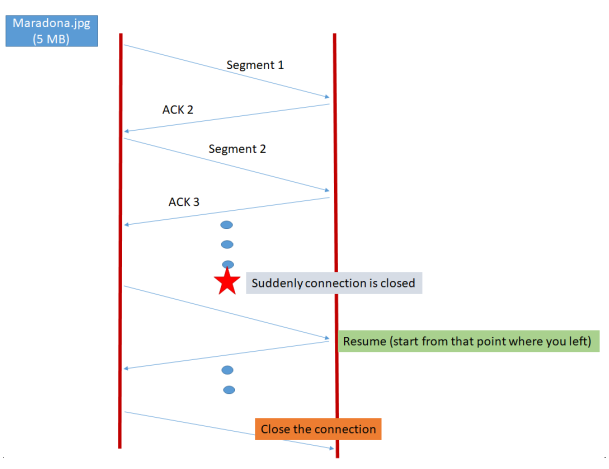
\includegraphics[width=350pt]{Question1Diagram}
\end{center}

Write a socket program in Java for Multimodal File Transmission using TCP and UDP with
\textbf{Full-Duplex Stop and Wait protocol}. The program/protocol should support the following
properties/mechanism
\begin{enumerate}
	\item The protocol will send any type of files
	\item Each packet should consist of the file name, sequence number/Acknowledgement
number
	\item A log file should be generated with some information like,
\end{enumerate}

List of uncommon files in server and client which are to be transferred, Start time, If
the connection is broken then the \% of the file already uploaded, How many times
connections were established during the complete transmission, End time (when the
file is fully transmitted), \textbf{How many packets are lost, How many time-outs are
occurred, etc.}
\pagebreak
\begin{flushleft}
\textbf{Answer.}
\end{flushleft}

The following code is the implementation for Multimodal File Transmission using TCP and UDP with
\textbf{Full-Duplex Stop and Wait protocol}.
\begin{lstlisting}

	Java Code:

\end{lstlisting}
\lstinputlisting[language=Java]{JavaCode/ReceiverClass.java}
\pagebreak
\lstinputlisting[language=Java]{JavaCode/SenderClass.java}
\pagebreak
\lstinputlisting[language=Java]{JavaCode/FileComparator.java}
\pagebreak
\lstinputlisting[language=Java]{JavaCode/Server.java}
\pagebreak
\lstinputlisting[language=Java]{JavaCode/Client.java}
\pagebreak

Output:


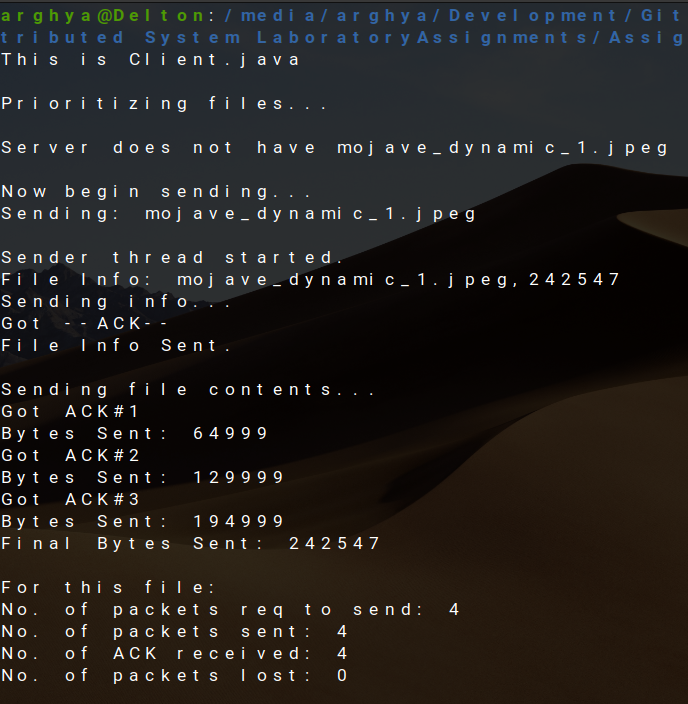
\includegraphics[width=365pt]{Output1}
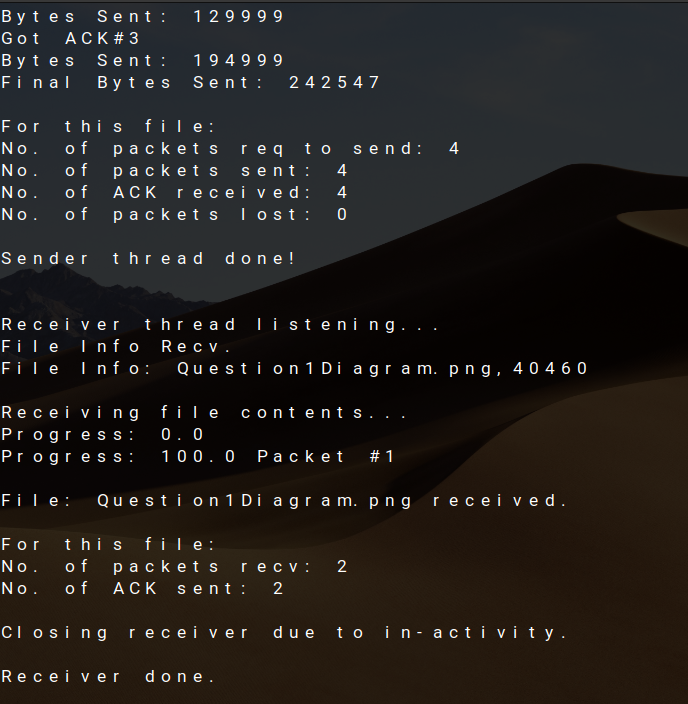
\includegraphics[width=365pt]{Output2}

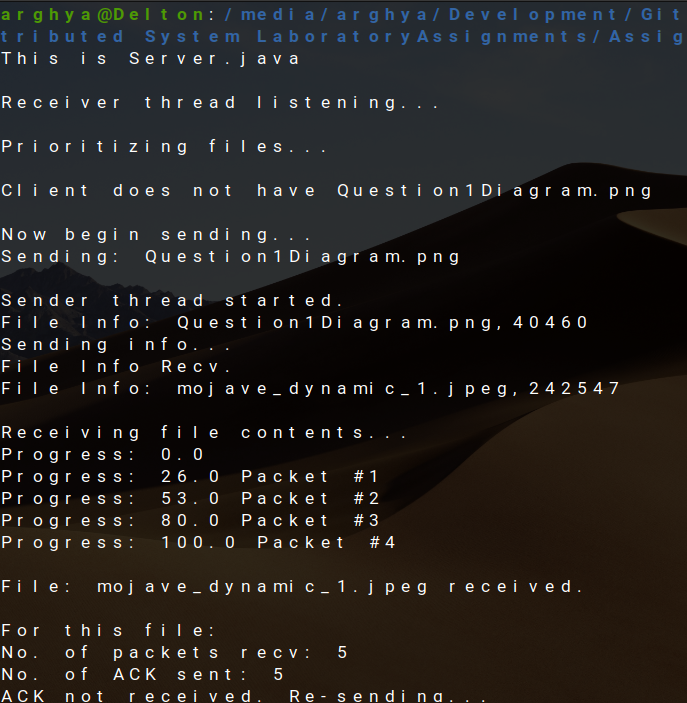
\includegraphics[width=365pt]{Output3}
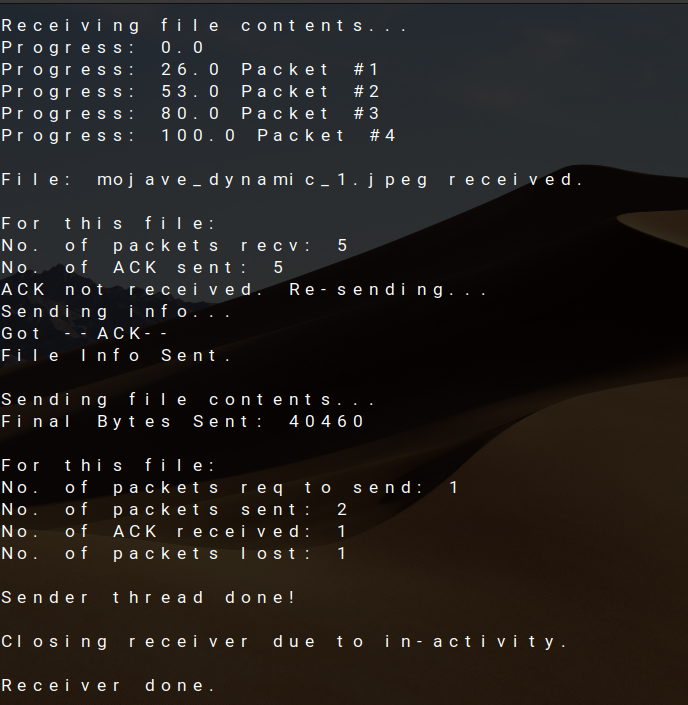
\includegraphics[width=365pt]{Output4}
\pagebreak

Log File

\begin{enumerate}
	\item Log File for the files in client files.
	\lstinputlisting{JavaCode/log_mojave_dynamic_1.jpeg.txt}
	\item Log File for the files in server files.
	\lstinputlisting{JavaCode/log_Question1Diagram.png.txt}
\end{enumerate}

\end{document}
